\documentclass{article}
\usepackage{anyfontsize}
\usepackage[UTF8]{ctex} % 如果需要支持中文
\usepackage{fontspec} 
\setCJKmainfont{SourceHanSansCN-Light}[
    BoldFont=SourceHanSansCN-Medium
]

\usepackage[a4paper, left=0.1in, right=0.1in, top=0.05in, bottom=0.05in]{geometry} % 设置四边页边距为0.1英寸{geometry} % 设置页边距为0.5英寸
\usepackage{enumitem} % 用于自定义列表
\usepackage{amsmath}  % 数学公式支持

\setlength{\parindent}{0pt} % 不缩进
\usepackage{etoolbox} % 用于列表操作
%调整类代码
\usepackage{comment}
\usepackage{tocloft} % 用于定制目录样式
%\usepackage{hyperref} %不需要目录盒子注释这
\usepackage{ifthen}
\usepackage{tikz}
\usepackage{titletoc}
\usepackage{graphicx}
\usepackage{amssymb}  % 提供数学符号，包括\therefore
\usepackage{multirow} 
\usepackage{pgfplots}
\usepackage{booktabs} % 用于表格的美观
\usepackage{float}  
\pgfplotsset{compat=1.15}
%目录设定
%快捷键 CMD + / 注释
%  \renewcommand{\cftdot}{} % 隐藏目录中的页码
%  \cftpagenumbersoff{section}
%  \cftpagenumbersoff{subsection}
%  \makeatletter
%  \renewcommand{\@pnumwidth}{0em}  % 设置页码宽度为0
%  \renewcommand{\@tocrmarg}{0em}   % 设置右边距为0
%  \makeatother
 


\usepackage{environ}

\newif\ifshowcontent  % 定义一个条件判断变量
\showcontenttrue    % 设置为 false，隐藏所有 question 环境的内容

\newcounter{question} % 题目计数器
\setcounter{question}{0}
\NewEnviron{question}{%
    \ifshowcontent
        \par\stepcounter{question}\textbf{\thequestion.} \BODY\par % 如果显示内容，则输出
    \fi
}

\NewEnviron{choices}{%
    \ifshowcontent
        \begin{enumerate}[label=\Alph*., leftmargin=*]
            \BODY
        \end{enumerate}\par
    \fi
}

\NewEnviron{correctanswer}{%
    \ifshowcontent
        \textbf{答案:}\BODY\par
    \fi
}



\newenvironment{explanation}
{\textbf{解析:}\par}
{\par}



% 新增考察方面命令
\newcommand{\checklist}[1]{
    \textbf{考察:} #1 \par % 在题目下方显示考察方面
    \addcontentsline{toc}{subsection}{题号\thequestion 考察: #1} % 将考察内容添加到目录
    \vspace{2em} % 添加1em的垂直空间
}

\graphicspath{{images/}} %统一


\begin{document}
 %\fontsize{23}{31}\selectfont
 \tableofcontents % 添加目录
\newpage
%\pagestyle{empty}





%模版
\section{考点1：Stationary Time Series 平稳的时间序列}
\setcounter{question}{0}

\begin{question}
    A junior analyst at a financial research firm is studying the concept of white noise in time - series analysis. Which of the following statements regarding white noise is false?
    \end{question}
    
    \begin{choices}
        \item If a process is stationary, has zero mean, has constant variance and is serially uncorrelated, then the process is white noise.
        \item If a process is Gaussian (aka, normal) white noise, then it must be independent white noise.
        \item If a process is Gaussian (aka, normal) white noise, then it must be (zero - mean) white noise.
        \item If a process is zero - mean white noise, then it must be Gaussian white noise.
    \end{choices}
    
    \begin{correctanswer}
        D
    \end{correctanswer}
    
    \begin{explanation}
    \textbf{A选项正确。}
    \begin{itemize}
        \item 根据白噪声的定义，一个平稳过程，具有零均值、常数方差且序列不相关，那么这个过程就是白噪声，故选项A正确。
    \end{itemize}
    \textbf{B选项正确。}
    \begin{itemize}
        \item 高斯白噪声是序列不相关且服从正态分布的白噪声，如果一个过程是高斯白噪声，那么它必然是独立白噪声，故选项B正确。
    \end{itemize}
    \textbf{C选项正确。}
    \begin{itemize}
        \item 高斯白噪声是白噪声的一种特殊情况，满足白噪声的基本特征，即零均值、常数方差和序列不相关，所以高斯白噪声一定是（零均值）白噪声，故选项C正确。
    \end{itemize}
    \textbf{D选项错误。}
    \begin{itemize}
        \item 零均值白噪声只要满足均值为零、方差恒定且序列不相关即可，不一定服从高斯分布。白噪声可以有多种分布形式，不一定是高斯分布，故选项D错误。
    \end{itemize}
    \end{explanation}
    
    \checklist{白噪声、高斯白噪声的性质（关键在于构成高斯白噪声需要满足的额外条件）}

\begin{question}
    A financial analyst at a hedge fund is studying time-series models. White noise is the fundamental building block of any time-series model. Which of the following statements about the properties of a white noise process is correct?
    \end{question}
    
    \begin{choices}
        \item Independent white noise is a special case of Gaussian white noise.
        \item In time-series modeling, the white noise process always follows a Poisson distribution.
        \item White noise is correlated over time and is necessarily independent.
        \item Any white noise process is covariance-stationary because the first two moments are time-invariant, and the variance is finite.
    \end{choices}
    
    \begin{correctanswer}
        D
    \end{correctanswer}
    
    \begin{explanation}
    \textbf{A选项错误。}
    \begin{itemize}
        \item 独立白噪声（观测值独立且不相关）比高斯白噪声（观测值独立且服从正态分布）更广义。高斯白噪声属于独立白噪声的特例，而非相反。
    \end{itemize}
    \textbf{B选项错误。}
    \begin{itemize}
        \item 白噪声过程不需要特定的分布假设，
    \end{itemize}
    \textbf{C选项错误。}
    \begin{itemize}
        \item 白噪声定义要求不相关，对独立性未作要求，仅独立白噪声要求具有独立性。
    \end{itemize}
    \textbf{D选项正确。}
    \begin{itemize}
        \item 白噪声满足协方差平稳三条件：均值恒定（\(E(\varepsilon_t)=0\)），方差恒定（\(Var(\varepsilon_t)=\sigma^2\)），自协方差仅与滞后阶数相关（\(Cov(\varepsilon_t,\varepsilon_{t-k})=0,\ \forall k\neq0\)）。
    \end{itemize}
    \end{explanation}
    
    \checklist{白噪声过程的性质（白噪声的不相关性、独立性、分布特征以及协方差平稳性等概念）}

\begin{question}
    A risk analyst at a prominent quantitative investment firm is delving into time - series analysis for portfolio optimization. As part of the process, the analyst is focusing on the concept of white noise, which is fundamental in understanding the randomness and predictability of financial time - series data. After conducting a series of tests and analyses, the analyst makes the following statements about white noise. Which statement is correct?
\end{question}
    
    \begin{choices}
        \item If \(\epsilon_t\) is serially uncorrelated, then we say \(\epsilon_t\) is independent white noise.
        \item Box - Pierce statistic could be used to test the null hypothesis that all its autocorrelations are jointly 0.
        \item Using Box - Pierce statistic \([Q_{BP}=T\sum_{\tau = 1}^{h}\hat{\rho}^{2}(\tau)]\) to test ARMA series, \(h\) is the higher the better if computational capacity is allowed.
        \item If one - step - ahead forecast errors contain white noise, the model should not be a preferred model.
    \end{choices}
    
    \begin{correctanswer}
    B
    \end{correctanswer}
    
    \begin{explanation}
    \textbf{A选项错误。}
    \begin{itemize}
    \item 仅序列不相关不能得出 \(\epsilon_t\) 是独立白噪声，独立白噪声除了序列不相关，还需满足均值为0、方差为常数且服从独立同分布等条件，该选项说法错误。
    \end{itemize}
    \textbf{B选项正确。}
    \begin{itemize}
    \item Box - Pierce统计量能够用于检验所有自相关系数联合为0的原假设，这是其常见应用，该选项说法正确。
    \end{itemize}
    \textbf{C选项错误。}
    \begin{itemize}
    \item 在使用Box - Pierce统计量检验ARMA序列时，虽然在计算能力允许下可以取较大的 \(h\) 以考虑更多滞后项，但并非 \(h\) 越高越好。过高的 \(h\) 可能会引入过多不必要的信息，导致检验结果不准确，该选项说法错误。
    \end{itemize}
    \textbf{D选项错误。}
    \begin{itemize}
    \item 一期预测误差包含白噪声是较好的模型的特征，该选项说法错误。
    \end{itemize}
    \end{explanation}
    
    \checklist{白噪声和Box - Pierce统计量（独立白噪声的性质和Box - Pierce统计量的原理）}

\begin{question}
    A risk analyst at an investment bank is performing a time - series analysis on bond yields. The analyst needs to determine if the time series is covariance stationary. Which of the following statements represents one of the requirements for a time series to be covariance stationary?
    \end{question}
    
    \begin{choices}
        \item When the autocovariance function is asymmetric with respect to displacement, \(\tau\), forward - looking stationarity can be achieved.
        \item The distribution of a time series should have a kurtosis value near 3.0, ensuring no fat tails will distort stationarity.
        \item The autocovariance of a covariance stationary time series depends only on displacement, \(\tau\), not on time.
        \item The distribution of a time series should have a skewness value near 0, so that its mean will fall in the center of the distribution.
    \end{choices}
    
    \begin{correctanswer}
        C
    \end{correctanswer}
    
    \begin{explanation}
    \textbf{A选项错误。}
    \begin{itemize}
        \item 协方差平稳性要求自协方差函数只与时间间隔\(\tau\)有关，而与时间无关，并且自协方差函数是关于位移\(\tau\)对称的。不对称的自协方差函数不符合协方差平稳的要求，也无法实现所谓的“前瞻性平稳性”，故选项A错误。
    \end{itemize}
    \textbf{B选项错误。}
    \begin{itemize}
        \item 协方差平稳性主要关注时间序列的均值、方差和自协方差的性质，与分布的峰度值没有直接关系，故选项B错误。
    \end{itemize}
    \textbf{C选项正确。}
    \begin{itemize}
        \item 对于一个协方差平稳的时间序列，其自协方差只依赖于时间间隔\(\tau\)，而不依赖于具体的时间点。也就是说，无论在哪个时间点进行观察，相同时间间隔的自协方差是恒定的，故选项C正确。
    \end{itemize}
    \textbf{D选项错误。}
    \begin{itemize}
        \item 协方差平稳性主要关注时间序列的均值、方差和自协方差的性质，与分布的偏度值没有直接关系，故选项D错误。
    \end{itemize}
    \end{explanation}
    
    \checklist{协方差平稳时间序列的3个性质（均值恒定、方差恒定且有限、自协方差有限且恒定，大小只和阶数有关）}

\begin{question}
    A risk analyst at a financial institution is comparing the moving average (MA) representation and the autoregressive (AR) process. Which of the following statements is a key differentiator between them?
    \end{question}
    
    \begin{choices}
        \item An autoregressive process is always covariance stationary.
        \item The structure of the MA(1) process has a longer memory than AR(1).
        \item A moving average representation shows evidence of autocorrelation cutoff.
        \item An autoregressive process shows evidence of autocorrelation cutoff.
    \end{choices}
    
    \begin{correctanswer}
        C
    \end{correctanswer}
    
    \begin{explanation}
    \textbf{A选项错误。}
    \begin{itemize}
        \item 自回归（AR）过程并不总是协方差平稳的。例如，对于 AR(1) 过程 \(Y_t=\phi Y_{t - 1}+\varepsilon_t\)，只有当 \(|\phi| < 1\) 时，该过程才是协方差平稳的。如果 \(|\phi|\geq1\)，过程就不满足协方差平稳的条件，其均值、方差和自协方差会随时间变化。
    \end{itemize}
    \textbf{B选项错误。}
    \begin{itemize}
        \item 移动平均（MA）过程的记忆是有限的。以 MA(1) 过程 \(Y_t=\mu+\varepsilon_t+\theta\varepsilon_{t - 1}\) 为例，它只依赖于当前和前一期的白噪声项，自相关函数在滞后大于 1 时为 0。而 AR(1) 过程 \(Y_t=\phi Y_{t - 1}+\varepsilon_t\) 的影响会无限期地传递下去，因为当前值 \(Y_t\) 依赖于前一期的值 \(Y_{t - 1}\)，而 \(Y_{t - 1}\) 又依赖于 \(Y_{t - 2}\) ，以此类推。所以 AR(1) 过程的记忆更长。
    \end{itemize}
    \textbf{C选项正确。}
    \begin{itemize}
        \item 移动平均（MA）表示的一个关键特征是自相关函数（ACF）会在某个滞后阶数之后截断。例如，对于 MA(q) 过程，其自相关函数在滞后 \(k > q\) 时为 0。这意味着该过程的自相关性在一定滞后阶数后消失，体现了自相关截断的特性。
    \end{itemize}
    \textbf{D选项错误。}
    \begin{itemize}
        \item 自回归（AR）过程的自相关函数不会截断，而是呈指数衰减。以 AR(1) 过程为例，其自相关函数 \(\rho(k)=\phi^k\)，随着滞后阶数 \(k\) 的增加，自相关系数逐渐减小，但不会突然截断为 0。
    \end{itemize}
    \end{explanation}
    
    \checklist{移动平均（MA）模型和自回归（AR）模型的区别（自相关截断、记忆长度和协方差平稳性等特性）}


\begin{question}
    A financial analyst at a hedge fund is looking to model seasonal stock price data. She is considering the use of an autoregressive (AR) process and an autoregressive moving average (ARMA) process. Which of the following statements correctly describes the usefulness of these two processes for this task?
    \end{question}
    
    \begin{choices}
        \item They both are mainly designed to handle the sudden shocks in time - series data.
        \item They both include lagged terms and, therefore, can better capture a relationship in motion.
        \item They both include the contemporaneous shocke,and the previous shock.
        \item They both specialize in capturing only the random movements in time series data.
    \end{choices}
    
    \begin{correctanswer}
        B
    \end{correctanswer}
    
    \begin{explanation}
    \textbf{A选项错误。}
    \begin{itemize}
        \item AR和ARMA模型主要是通过包含滞后项来捕捉时间序列中的自相关关系，而不是专门用于处理时间序列数据中的突发冲击。突发冲击通常更适合用ARCH、GARCH等模型来处理，故选项A错误。
    \end{itemize}
    \textbf{B选项正确。}
    \begin{itemize}
        \item AR模型包含滞后的因变量项，ARMA模型既包含滞后的因变量项又包含滞后的误差项。这些滞后项使得模型能够捕捉到时间序列中变量之间随时间变化的动态关系，也就是所谓的“动态中的关系”，故选项B正确。
    \end{itemize}
    \textbf{C选项错误。}
    \begin{itemize}
        \item AR模型不包含滞后的误差项，MA模型和ARMA模型包含滞后的误差项，所以选项C错误。
    \end{itemize}
    \textbf{D选项错误。}
    \begin{itemize}
        \item AR和ARMA模型不仅仅是捕捉时间序列中的随机运动。它们通过对滞后项的建模，能够揭示时间序列中的自相关结构和潜在的规律，而不是只关注随机部分，故选项D错误。
    \end{itemize}
    \end{explanation}
    
    \checklist{AR模型和ARMA模型的特点（理解模型中包含哪些滞后项）}

\begin{question}
    A risk analyst at a leading investment firm, Alex Thompson, is looking into modeling the cyclical stock returns of a tech company. Considering using AR(1) and MA(1) models, he makes the following statements about the characteristics of these models before building them. Which statement is most likely incorrect?
    \end{question}
    
    \begin{choices}
        \item The AR(1) model is \(y_t=\delta+\varphi\times y_{t - 1}+\epsilon_t\) and if the absolute value of \(\varphi\) is less than 1, the AR(1) model is covariance stationary.
        \item The MA(1) model is \(y_t=\mu+\epsilon_t+\theta\times\epsilon_{t - 1}\) and no matter what value \(\theta\) takes,  the MA(1) process is always covariance stationary.
        \item The ACF (autocorrelation function) of AR(1) process decays as the time lag length increases and the PACF (partial autocorrelation function) decays as the time lag length increases.
        \item The ACF (autocorrelation function) of MA(1) process cuts off as the time lag length increases and the PACF (partial autocorrelation function) decays as the time lag length increases.
    \end{choices}
    
    \begin{correctanswer}
    C
    \end{correctanswer}
    
    \begin{explanation}
    \textbf{A选项正确。}
    \begin{itemize}
    \item AR(1)模型 \(y_t=\delta+\varphi\times y_{t - 1}+\epsilon_t\)，当\(|\varphi|<1\)时，满足自回归过程平稳的条件，此时该模型是协方差平稳的，该选项说法正确。
    \end{itemize}
    \textbf{B选项正确。}
    \begin{itemize}
    \item MA(1)模型 \(y_t=\mu+\epsilon_t+\theta\times\epsilon_{t - 1}\)，其均值、方差和自协方差不依赖于时间\(t\)，无论\(\theta\)取何值，MA(1)过程总是协方差平稳的，该选项说法正确。
    \end{itemize}
    \textbf{C选项错误。}
    \begin{itemize}
    \item AR(1)模型的自相关函数(ACF)随着滞后阶数的增大而逐渐衰减(decay)到 0,偏自相关系数(PACF)随着滞后阶数的增大而直接降低到0，有截尾特征，并非随着滞后长度增加而截断，该选项说法错误。
    \end{itemize}
    \textbf{D选项正确。}
    \begin{itemize}
    \item MA(1)模型的自相关函数(ACF)随着滞后阶数的增大直接降低到 0，有截尾特征，偏自相关系数(PACF)随着滞后阶数的增大面逐渐衰减到0，该选项说法正确。
    \end{itemize}
    \end{explanation}
    
    \checklist{AR(1)和MA(1)模型（关键在区分两种模型协方差平稳的条件以及与ACF和PACF的关系）}

\begin{question}
    A risk analyst at a fixed - income investment firm is analyzing a covariance - stationary ARMA(1, 1) model. The model is given by \(Y_t = 0.5 + 0.4Y_{t - 1}-0.7\epsilon_{t - 1}+\epsilon_t\), where \(\epsilon_t\sim WN(0,\sigma^2)\). What is the long - run mean \(E[Y_t]\)?
    \end{question}
    
    \begin{choices}
        \item \(E[Y_t]= - 1.67\)
        \item \(E[Y_t]=0.71\)
        \item \(E[Y_t]=0.83\)
        \item \(E[Y_t]= - 0.45\)
    \end{choices}
    
    \begin{correctanswer}
        C
    \end{correctanswer}
    
    \begin{explanation}
    \textbf{步骤1：明确长期均值的性质。}
    \begin{itemize}
        \item 在协方差平稳的时间序列中，长期均值 \(E[Y_t]\) 是一个常数，即 \(E[Y_t]=E[Y_{t - 1}]\)，并且 \(E[\epsilon_t]=0\)，\(E[\epsilon_{t - 1}]=0\)。
    \end{itemize}
    \textbf{步骤2：对给定的ARMA(1, 1)模型取期望。}
    \begin{itemize}
        \item 对 \(Y_t = 0.5 + 0.4Y_{t - 1}-0.7\epsilon_{t - 1}+\epsilon_t\) 两边同时取期望，得到 \(E[Y_t]=0.5 + 0.4E[Y_{t - 1}]-0.7E[\epsilon_{t - 1}]+E[\epsilon_t]\)。
        \item 由于 \(E[\epsilon_t]=0\)，\(E[\epsilon_{t - 1}]=0\)，且 \(E[Y_t]=E[Y_{t - 1}]\)，设 \(E[Y_t]=\mu\)，则方程变为 \(\mu = 0.5+0.4\mu\)。
    \end{itemize}
    \textbf{步骤3：求解长期均值 \(\mu\)。}
    \begin{itemize}
        \item 对 \(\mu = 0.5 + 0.4\mu\) 进行移项可得：\(\mu-0.4\mu=0.5\)，即 \(0.6\mu = 0.5\)。
        \item 解得 \(\mu=\frac{0.5}{0.6}=0.83\)。
    \end{itemize}
    \end{explanation}
    
    \checklist{ARMA(1, 1)模型长期均值的计算（\(E[Y_t] = \mu = \delta / (1 - \phi)\)）}


\begin{question}
    A risk analyst at an asset management firm is trying to analyze and forecast the performance of a particular stock. The analyst has gathered the historical time - series data of the stock. Based on the Partial Autocorrelation Function (PACF) plot shown below, which of the following is the most appropriate regression approach for this stock?

    \end{question}
    \begin{figure}[h]
        \centering
        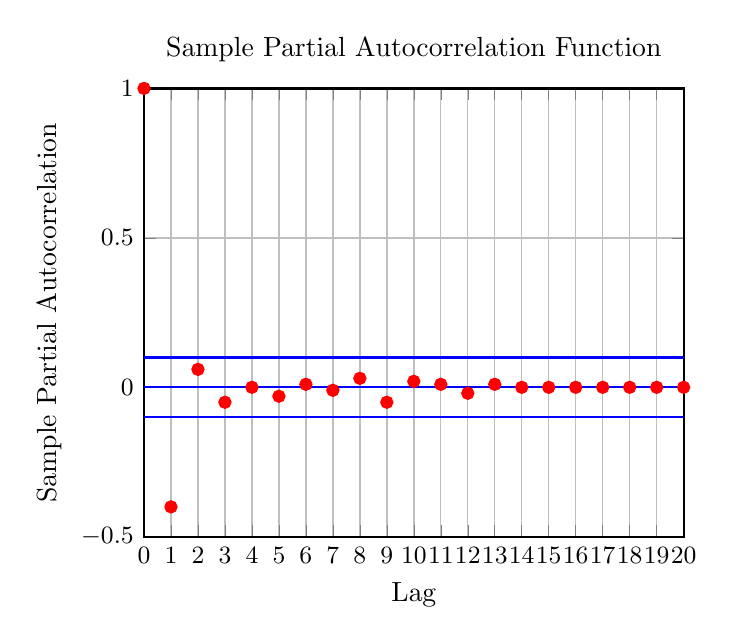
\begin{tikzpicture}
            \begin{axis}[
                title={Sample Partial Autocorrelation Function},
                xlabel={Lag},
                ylabel={Sample Partial Autocorrelation},
                ymin=-0.5, ymax=1,
                xmin=0, xmax=20,
                xtick={0,1,...,20},
                ytick={-0.5,0,0.5,1},
                grid=both,
                major grid style={line width=.5pt,draw=gray!50},
                minor grid style={line width=.5pt,draw=gray!20},
                thick,
                every axis label/.append style={font=\normalsize},
                every tick label/.append style={font=\small},
            ]
            % PACF values for AR(1) model
            \addplot[only marks, mark=*, red] coordinates {
                (0, 1) (1, -0.4) (2, 0.06) (3, -0.05) (4, 0) (5, -0.03)
                (6, 0.01) (7, -0.01) (8, 0.03) (9, -0.05) (10, 0.02)
                (11, 0.01) (12, -0.02) (13, 0.01) (14, 0) (15, 0)
                (16, 0) (17, 0) (18, 0) (19, 0) (20, 0)
            };
            % Confidence intervals
            \addplot[blue, thick] coordinates {(0, 0.1) (20, 0.1)};
            \addplot[blue, thick] coordinates {(0, -0.1) (20, -0.1)};
            \addplot[blue, thick] coordinates {(0, 0) (20, 0)};
            \end{axis}
        \end{tikzpicture}
    \end{figure}
    \begin{choices}
        \item MA(2)
        \item AR(1)
        \item MA(1)
        \item AR(2)
    \end{choices}
    
    \begin{correctanswer}
        D
    \end{correctanswer}
    
    \begin{explanation}
    PACF图主要用于判断AR模型的阶数，该题中的PACF图在二阶后截尾，故应选择AR(2)模型，选项D正确。MA（移动平均）模型的阶数通常根据自相关函数（ACF）来确定，而不是偏自相关函数（PACF）。

    \textbf{ACF \& PACF Summary:}
    \begin{center}
        \begin{tabular}{|c|c|c|}
            \hline
            Model & ACF & PACF \\ \hline
            AR & 拖尾 decay & 截尾 cutoff \\ \hline
            MA & 截尾 cutoff & 拖尾 decay \\ \hline
            ARMA & 拖尾 decay & 拖尾 decay \\ \hline
        \end{tabular}
    \end{center}
    \end{explanation}
    
    \checklist{根据偏自相关函数（PACF）图确定适用的模型及模型阶数（PACF图截尾应选用AR模型）}


    \begin{question}
        A risk analyst at a financial institution is working on a covariance - stationary ARMA(2, 2) model. The model is defined as \(Y_t = 0.3+0.5Y_{t - 1}-0.2Y_{t - 2}+0.7\epsilon_{t - 1}+0.2\epsilon_{t - 2}+\epsilon_t\), where \(\epsilon_t\sim WN(0,\sigma^2)\). What is the long - run unconditional mean of \(Y_t\)?
        \end{question}
        
        \begin{choices}
            \item \(1.5\)
            \item \(0.3333\)
            \item \(0.4286\)
            \item \(2\)
        \end{choices}
        
        \begin{correctanswer}
            C
        \end{correctanswer}
        
        \begin{explanation}
        \textbf{步骤1：明确长期均值的性质。}
        \begin{itemize}
            \item 在协方差平稳的时间序列中，长期均值 \(E[Y_t]\) 是一个常数，即 \(E[Y_t]=E[Y_{t - 1}]=E[Y_{t - 2}]\)，并且 \(E[\epsilon_t]=0\)，\(E[\epsilon_{t - 1}]=0\)，\(E[\epsilon_{t - 2}]=0\)。
        \end{itemize}
        \textbf{步骤2：对给定的ARMA(2, 2)模型取期望。}
        \begin{itemize}
            \item 对 \(Y_t = 0.3+0.5Y_{t - 1}-0.2Y_{t - 2}+0.7\epsilon_{t - 1}+0.2\epsilon_{t - 2}+\epsilon_t\) 两边同时取期望，得到 \(E[Y_t]=0.3 + 0.5E[Y_{t - 1}]-0.2E[Y_{t - 2}]+0.7E[\epsilon_{t - 1}]+0.2E[\epsilon_{t - 2}]+E[\epsilon_t]\)。
            \item 由于 \(E[\epsilon_t]=0\)，\(E[\epsilon_{t - 1}]=0\)，\(E[\epsilon_{t - 2}]=0\)，且 \(E[Y_t]=E[Y_{t - 1}]=E[Y_{t - 2}]\)，设 \(E[Y_t]=\mu\)，则方程变为 \(\mu = 0.3+0.5\mu - 0.2\mu\)。
        \end{itemize}
        \textbf{步骤3：求解长期均值 \(\mu\)。}
        \begin{itemize}
            \item 对 \(\mu = 0.3+0.5\mu - 0.2\mu\) 进行移项可得：\(\mu-0.5\mu + 0.2\mu=0.3\)，即 \(0.7\mu = 0.3\)。
            \item 解得 \(\mu=\frac{0.3}{0.7}=\frac{3}{7}\approx0.4286\)。
        \end{itemize}
        \end{explanation}
        
        \checklist{ARMA(2, 2)模型长期均值的计算（掌握自回归项和移动平均项的期望性质）}

\begin{question}
    A junior risk analyst at a hedge fund is attempting to forecast the expected return of a stock using the following AR(1) model: \(y_t = 1.67 + 0.65y_{t - 1}+\epsilon_t\). The analyst is puzzled about the significant impacts of covariance stationarity on the forecasting model and the implications of the model. Which of the following statements regarding the analyst's concern is most likely incorrect?
    \end{question}
    
    \begin{choices}
        \item The long - run forecast from the time series is 4.77, which is equal to the mean reversion level of the AR(1) model.
        \item The model constructed by the analyst is covariance - stationary, because \(\vert\phi_1\vert=\vert0.65\vert < 1\).
        \item The AR(1) model relates the current value of a stochastic process (i.e., \(y_t\)) to its value two periods ago (i.e., \(y_{t - 2}\)).
        \item A covariance - stationary time series implies a constant relationship across time, allowing historical data to be used to estimate models that are applicable to future out - of - sample observations.
    \end{choices}
    
    \begin{correctanswer}
        C
    \end{correctanswer}
    
    \begin{explanation}
    
    \textbf{A选项正确。}
    \begin{itemize}
        \item 对于AR(1)模型 \(y_t=\phi_0+\phi_1y_{t - 1}+\epsilon_t\)，其长期均值（即均值回归水平）的计算公式为 \(\mu=\frac{\phi_0}{1 - \phi_1}\)。
        \item 已知 \(\phi_0 = 1.67\)，\(\phi_1 = 0.65\)，代入可得 \(\mu=\frac{1.67}{1 - 0.65}=4.77\)，长期预测值等于均值回归水平。所以该选项描述正确。
    \end{itemize}
    \textbf{B选项正确。}
    \begin{itemize}
        \item AR(1)模型 \(y_t=\phi_0+\phi_1y_{t - 1}+\epsilon_t\) 具有协方差平稳性的条件是自回归系数 \(\phi_1\) 的绝对值小于1。
        \item 在本题中 \(\vert\phi_1\vert=\vert0.65\vert < 1\)，所以该模型是协方差平稳的。该选项描述正确。
    \end{itemize}
    \textbf{C选项错误。}
    \begin{itemize}
        \item 自回归一阶模型（AR(1)）的形式为 \(y_t=\phi_0+\phi_1y_{t - 1}+\epsilon_t\)，它是将当前时刻的随机过程值 \(y_t\) 与前一时刻的值 \(y_{t - 1}\) 相关联，而不是与前两期的值 \(y_{t - 2}\) 相关联。所以该选项描述错误。
    \end{itemize}
    \textbf{D选项正确。}
    \begin{itemize}
        \item 协方差平稳的时间序列意味着其均值、方差和自协方差不随时间变化，具有恒定的关系。
        \item 基于这种特性，我们可以利用历史数据来估计模型参数，并且这些模型对于未来的样本外观测值也是适用的。所以该选项描述正确。
    \end{itemize}
    \end{explanation}
    
    \checklist{AR(1)模型的性质（理解AR(1)模型的形式、协方差平稳的条件和长期均值的计算公式）}


\begin{question}
    A risk analyst at an investment firm is analyzing a time series that consists of thirty - six quarterly observations (\(m = \text{degrees of freedom}=36\)). The analyst has calculated the Box - Pierce Q - statistic to be 28.80 and the Ljung - Box Q - statistic to be 38.20. The analyst wants to determine if the series is white noise. Given that \(\text{CHISQ.INV}(0.95, 36)=50.99\), which of the following is the best conclusion?
    \end{question}
    
    \begin{choices}
        \item With 95\% confidence, you accept the series as white noise (more accurately, you fail to reject the null).
        \item With 95\% confidence, you accept the series as partial white noise (due to Box - Pierce) but reject the null (due to Ljung - Box).
        \item With 95\% confidence, you reject both null hypotheses and conclude the series is not white noise.
        \item With 95\% confidence, you reject both null hypotheses but conclude the series is white noise because the sum of the statistics is greater than the critical value.
    \end{choices}
    
    \begin{correctanswer}
        A
    \end{correctanswer}
    
    \begin{explanation}
    \textbf{Joint Tests of Autocorrelations：}
    \begin{itemize}
        \item 在检验时间序列是否为白噪声时，原假设 \(H_0\) 是该时间序列是白噪声。使用Box - Pierce和Ljung - Box Q统计量进行检验，当计算得到的Q统计量小于临界值时，我们不能拒绝原假设。
        \item 已知自由度 \(m = 36\)，\(\text{CHISQ.INV}(0.95, 36)=50.99\) 为临界值，计算得到的Box - Pierce Q统计量为28.80，Ljung - Box Q统计量为38.20，两者均小于临界值50.99。
        \item 所以，在95\%的置信水平下，我们不能拒绝原假设，即接受该序列为白噪声，故选项A正确。
    \end{itemize}
    \end{explanation}
    
    \checklist{使用Box - Pierce和Ljung - Box Q统计量检验时间序列是否为白噪声（比较Q统计量与临界值的大小）}

    \begin{question}
        A risk analyst at a financial research firm is conducting a specification analysis on an ARMA model by testing autocorrelation in the residuals. The analyst is considering the two closely - related tests: the Box - Pierce test and the Ljung - Box test. Which of the following statements accurately differentiates these two tests?
        \end{question}
        
        \begin{choices}
            \item Under both tests, a rejection of the null hypothesis indicates that the model fails to account for certain dynamics in a time series.
            \item They have the same null hypothesis, which posits that all autocorrelations are non-zero.
            \item The Box - Pierce test performs better in smaller samples compared to the Ljung - Box test.
            \item Asymptotically, the Ljung - Box test - statistic follows a normal distribution, while the Box - Pierce test - statistic follows a chi - squared distribution.
        \end{choices}
        
        \begin{correctanswer}
            A
        \end{correctanswer}
        
        \begin{explanation}
        \textbf{A选项正确。}
        \begin{itemize}
            \item 对于Box - Pierce检验和Ljung - Box检验，原假设 \(H_0\) 是残差序列的自相关系数都为零，即模型已经捕捉了时间序列的所有动态特征。
            \item 当拒绝原假设时，意味着至少存在一个自相关系数不为零，即原模型不能解释时间序列中的自相关结构，说明模型未能捕捉到时间序列中的某些动态特征，故选项A正确。
        \end{itemize}
        \textbf{B选项错误。}
        \begin{itemize}
            \item 两个检验的原假设是所有自相关系数都为零，而不是“所有自相关系数不为零”，故选项B错误。
        \end{itemize}
        \textbf{C选项错误。}
        \begin{itemize}
            \item 通常Ljung - Box检验在小样本下比Box - Pierce检验更有效，故选项C错误。
        \end{itemize}
        \textbf{D选项错误。}
        \begin{itemize}
            \item 渐近情况下，Box - Pierce检验统计量和Ljung - Box检验统计量都服从卡方分布，故选项D错误。
        \end{itemize}
        \end{explanation}

        \checklist{区分Box - Pierce检验和Ljung - Box检验（掌握两个检验的原假设、小样本适用性及统计量分布特点）}

\begin{question}
    A data analyst at a financial firm is using the Box-Pierce and Ljung-Box Q-statistics to analyze time-series data. Which of the following statements about these statistics is false?
    \end{question}
    
    \begin{choices}
        \item The Box-Pierce Q-statistic is used to test whether the residuals in a time series are white noise.
        \item The Ljung-Box Q-statistic is used to test for a linear trend in a time series under the null hypothesis of a unit root.
        \item Under the null hypothesis that autocorrelations are jointly zero in a time series, the Box-Pierce Q-statistic is approximately distributed as a chi-squared random variable.
        \item In the Ljung-Box test, the selection of the number of lags being tested is a balance between conducting a joint test and the quality of the distribution approximations.
    \end{choices}
    
    \begin{correctanswer}
        B
    \end{correctanswer}
    
    \begin{explanation}
    \textbf{A选项正确。}
    \begin{itemize}
        \item Box-Pierce Q统计量的核心用途是检验时间序列残差是否为白噪声，通过检验自相关系数的联合显著性来判断模型是否充分。
    \end{itemize}
    \textbf{B选项错误。}
    \begin{itemize}
        \item Ljung-Box检验的原假设是前m阶自相关系数均为零，与单位根无关。单位根检验需使用ADF或PP检验，线性趋势检测则通过回归分析实现。
    \end{itemize}
    \textbf{C选项正确。}
    \begin{itemize}
        \item Box-Pierce统计量在零假设下渐近服从\(\chi^2(m)\)分布，其中m为滞后阶数。
    \end{itemize}
    \textbf{D选项正确。}
    \begin{itemize}
        \item 滞后阶数m的选择需权衡：m过小可能遗漏高阶自相关，m过大会降低卡方近似的准确性，通常取\(m \approx \ln(T)\)（T为样本量）。
    \end{itemize}
    \end{explanation}
    
    \checklist{Box-Pierce和Ljung-Box Q统计量的应用和性质（核心是检验目的、分布特性及滞后阶数选择）}


\begin{question}
In financial risk management (FRM), autocorrelation function (ACF) and partial autocorrelation function (PACF) are important tools for analyzing time series data. Based on the provided material, which of the following statements is incorrect?
\end{question}

\begin{choices}
    \item The autocorrelation function (ACF) is calculated by dividing the autocovariance by the variance of the time series, resulting in values between -1 and +1.
    \item For a covariance-stationary time series, ACF values tend to approach zero as the time lag τ increases.
    \item The partial autocorrelation function (PACF) measures the predictive ability of a single lag on the time series after controlling for the effects of all other lags.
    \item In partial autocorrelation analysis, all PACF values gradually decrease as the time lag τ increases.
\end{choices}

\begin{correctanswer}
D
\end{correctanswer}

\begin{explanation}
\textbf{A选项正确。}
\begin{itemize}
    \item 自相关函数（ACF）是通过将自协方差除以时间序列的方差来标准化的：
    \[\rho(k) = \frac{\gamma(k)}{\gamma(0)}\]
    其中 \(\gamma(k)\) 是k阶自协方差，\(\gamma(0)\) 是方差
    \item 这种标准化使得ACF值必然落在[-1, 1]区间内。
\end{itemize}

\textbf{B选项正确。}
\begin{itemize}
    \item 对于协方差平稳的时间序列，随着滞后阶数k的增加，序列之间的相关性会逐渐减弱。
    \item 这种特性反映在ACF上就是：\(\lim_{k \to \infty} \rho(k) = 0\)
\end{itemize}

\textbf{C选项正确。}
\begin{itemize}
    \item PACF衡量的是在控制了中间所有滞后项（\(Y_{t-1}, Y_{t-2}, ..., Y_{t-k+1}\)）的影响后。\(Y_t\) 与 \(Y_{t-k}\) 之间的相关性，反映了纯粹的k阶滞后效应。
\end{itemize}

\textbf{D选项错误。}
\begin{itemize}
    \item PACF值不一定随着滞后阶数增加而缓慢减小，对于AR(p)过程，PACF在p阶后会突然截断为0，对于MA(q)过程，PACF会呈指数衰减。
    \item PACF值可能在某些特定的滞后值上显著，而在其他滞后值上迅速减小。
\end{itemize}
\end{explanation}

\checklist{自相关函数（ACF）和偏自相关函数（PACF）的特性（PACF值可能在某些特定的滞后值上显著，而在其他滞后值上迅速减小。）}



\begin{question}
    A quantitative analyst at a hedge fund is developing time series models to forecast asset returns. While examining both AR(1) and MA(1) models for different financial instruments, she needs to understand the properties of autocorrelation function (ACF) and partial autocorrelation function (PACF) to select the most appropriate model. Based on her analysis of these models, which of the following statements is CORRECT?
    \end{question}
    
    \begin{choices}
        \item The AR(1) model \(Y_t = \delta + \varphi Y_{t-1} + \epsilon_t\) she has tested is covariance-stationary when \(|\varphi| < 1\).
        \item The MA(1) model requires the condition \(|\theta| < 1\) to ensure its covariance stationarity.
        \item The PACF plots she generated for the MA(1) model exhibit a sharp cut-off pattern after lag 1.
        \item The ACF plots she generated for the AR(1) model show a cut-off pattern after lag 1.
    \end{choices}
    
    \begin{correctanswer}
    A
    \end{correctanswer}
    
    \begin{explanation}
    \textbf{A选项正确。}
    \begin{itemize}
        \item 这个陈述准确描述了AR(1)模型的平稳性条件。
        \item AR(1)模型必须在\(|\varphi| < 1\)时才平稳，这是保证过去的冲击不会无限累积的必要条件。
        \item 当\(|\varphi| \geq 1\)时，序列的方差会无限增大，违反平稳性要求。
    \end{itemize}
    
    \textbf{B选项错误。}
    \begin{itemize}
        \item MA(1)模型对任意参数值\(\theta\)都是协方差平稳的，不需要\(|\theta| < 1\)的条件。
        \item 这是因为MA过程是有限个白噪声的线性组合，而白噪声过程具有固定的均值和方差。
    \end{itemize}
    
    \textbf{C选项错误。}
    \begin{itemize}
        \item MA(1)模型的PACF实际上呈现衰减模式，而不是截尾模式。
        \item 这是MA(1)模型的一个重要特征，可以用来识别时间序列的类型。
    \end{itemize}
    
    \textbf{D选项错误。}
    \begin{itemize}
        \item AR(1)模型的ACF实际上呈现衰减模式，而不是截尾模式。
        \item 这种衰减模式反映了AR(1)过程中，过去观测值的影响会随时间逐渐减弱。
    \end{itemize}
    
    \begin{center}
    \begin{tabular}{|c|c|c|}
    \hline
    模型 & ACF & PACF \\
    \hline
    MA(1)模型 & 截尾(cut off) & 衰减(decay) \\
    \hline
    AR(1)模型 & 衰减(decay) & 截尾(cut off) \\
    \hline
    \end{tabular}
    \end{center}
    
    \end{explanation}
    
    \checklist{时间序列模型的平稳性条件和自相关特征（ACF和PACF的模式特征）}

\section{考点2：Non-Stationary Time Series 非平稳的时间序列}
\setcounter{question}{0}
\begin{question}
    An analyst at a retail consulting firm, Lily, is building a model to predict a client's sales over time. She has identified a quarterly seasonal pattern in the sales data. If Lily includes an intercept term in her model, how many dummy variables should she use to model the seasonality component?
    \end{question}
    
    \begin{choices}
        \item 5
        \item 4
        \item 2
        \item 3
    \end{choices}
    
    \begin{correctanswer}
        D
    \end{correctanswer}
    
    \begin{explanation}
    在回归模型中，当存在截距项时，对于具有 \(n\) 个类别的分类变量，需要使用 \(n - 1\) 个虚拟变量来避免多重共线性。这里季节有4个类别，所以应该使用 \(4-1 = 3\) 个虚拟变量来建模季节成分，选项D正确。
    \end{explanation}
    
    \checklist{时间序列的季节性（虚拟变量数量等于分类变量类别数减1）}

    \begin{question}
        A financial analyst at a consumer goods company is using a regression model with dummy variables to analyze quarterly sales. The regression equation is \(SALES_t = \beta_0+\beta_2D_{2,t}+\beta_3D_{3,t}+\beta_4D_{4,t}+\epsilon_t\), where \(SALES_t\) is a quarterly observation of sales, \(D_{2,t} = 1\) if period \(t\) is the second quarter and \(0\) otherwise, \(D_{3,t} = 1\) if period \(t\) is the third quarter and \(0\) otherwise, and \(D_{4,t} = 1\) if period \(t\) is the fourth quarter and \(0\) otherwise. The intercept term \(\beta_0\) represents the average value of sales for the:
        \end{question}
        
        \begin{choices}
            \item Fourth quarter
            \item Second quarter
            \item First quarter
            \item Third quarter
        \end{choices}
        
        \begin{correctanswer}
            C
        \end{correctanswer}
        
        \begin{explanation}
        \textbf{A选项错误。}
        \begin{itemize}
            \item 当处于第四季度时，\(D_{4,t}=1\)，此时销售的平均值为\(\beta_0 + \beta_4\)，并非\(\beta_0\)，所以该选项错误。
        \end{itemize}
        \textbf{B选项错误。}
        \begin{itemize}
            \item 当处于第二季度时，\(D_{2,t}=1\)，销售的平均值为\(\beta_0+\beta_2\)，不是\(\beta_0\)，所以该选项错误。
        \end{itemize}
        \textbf{C选项正确。}
        \begin{itemize}
            \item 在这个回归模型中，没有为第一季度设置虚拟变量。当所有虚拟变量\(D_{2,t}=D_{3,t}=D_{4,t}=0\)时，即代表第一季度，此时回归方程变为\(SALES_t=\beta_0+\epsilon_t\)，所以截距项\(\beta_0\)代表第一季度销售的平均值。
        \end{itemize}
        \textbf{D选项错误。}    
        \begin{itemize}
            \item 当处于第三季度时，\(D_{3,t}=1\)，销售的平均值为\(\beta_0+\beta_3\)，不是\(\beta_0\)，所以该选项错误。
        \end{itemize}
        \end{explanation}
        
        \checklist{虚拟变量在回归模型中的含义（理解未设置虚拟变量的类别对应的是截距项所代表的情况）}







\begin{question}
    A risk analyst at a financial forecasting firm is evaluating different scenarios for building a forecasting model. Which of the following scenarios would lead to a forecasting model that exhibits perfect multicollinearity?
    \end{question}
    
    \begin{choices}
        \item A model that includes a trading - day variation variable for modeling trading volume throughout the year.
        \item A model that includes a holiday variation variable that accounts for an “Easter dummy variable.”
        \item A model that includes only one seasonal dummy that is equal to 1.
        \item A model that includes a dummy variable for each season, plus an intercept.
    \end{choices}
    
    \begin{correctanswer}
        D
    \end{correctanswer}
    
    \begin{explanation}
    \textbf{A选项错误。}
    \begin{itemize}
        \item 交易天数变化变量用于模拟全年的交易量，它本身不会导致模型出现完全多重共线性。该变量可以合理地解释交易量随交易天数的变化，不存在与其他变量之间的线性依赖关系，所以该选项错误。
    \end{itemize}
    \textbf{B选项错误。}
    \begin{itemize}
        \item 包含复活节虚拟变量的假日变化变量，它只是用来捕捉假日对模型的影响，一般不会与其他变量产生完全的线性关系，不会导致完全多重共线性，所以该选项错误。
    \end{itemize}
    \textbf{C选项错误。}
    \begin{itemize}
        \item 仅包含一个始终等于1的季节性虚拟变量，它不会与其他变量产生完全的线性组合关系，不会造成完全多重共线性，所以该选项错误。
    \end{itemize}
    \textbf{D选项正确。}
    \begin{itemize}
        \item 在回归模型中，如果为每个季节都设置一个虚拟变量，再加上截距项，就会出现完全多重共线性。因为季节虚拟变量的和是一个常数（如果有4个季节，4个虚拟变量之和始终为1），再加上截距项，就会导致变量之间存在精确的线性关系，使得模型无法准确估计参数。
    \end{itemize}
    \end{explanation}
    
    \checklist{回归模型中完全多重共线性的判断（虚拟变量数量设置不当会导致多重共线性）}


\begin{question}
    A financial analyst at an investment firm is examining the Augmented Dickey - Fuller (ADF) test results for the growth rate of real GDP to determine whether a unit root exists. The figure below shows the ADF test results. Column $\gamma$ reports the parameter estimate from the ADF test regression and the ADF statistic (in parentheses). The columns $\delta_0$ and $\delta_1$ report estimates of the constant and linear trend along with t - Statistics. The final column reports the 5\% critical values. Which of the following statements is correct?
    \begin{center}
    \begin{tabular}{|c|c|c|c|c|}
    \hline 
    Deterministic & $\gamma$ & $\delta_0$ & $\delta_1$ & 5\% CV \\ 
    \hline 
    Trend & -0.856 (-9.234) & 9.12e-03 (6.321) & -1.65e-05 (-2.567) & -3.512 \\ 
    \hline 
    \end{tabular}
    \end{center}
    \end{question}
    
    \begin{choices}
        \item An ADF test will reject the hypothesis that a process is a unit root if the coefficient on the lagged value is statistically significantly equal to zero.
        \item The real GDP growth rate does not contain a unit root.
        \item The real GDP growth rate does contain a unit root.
        \item The real GDP growth rate is covariance stationary as $\gamma$ is significantly equal to zero.
    \end{choices}
    
    \begin{correctanswer}
    B
    \end{correctanswer}
    
    \begin{explanation}
    \textbf{A选项错误。}
    \begin{itemize}
    \item 在ADF检验中，原假设是存在单位根，备择假设是不存在单位根。如果滞后值的系数统计显著地小于零，才会拒绝存在单位根的原假设，而不是等于零，所以A选项错误。 
    \end{itemize}
    \textbf{B选项正确。}
    \begin{itemize}
    \item ADF统计量为 -9.234，5\%的临界值为 -3.512，ADF统计量的绝对值大于临界值的绝对值，故应拒绝原假设（存在单位根），实际GDP增长率不包含单位根，B选项正确。 
    \end{itemize}
    \textbf{C选项错误。}
    \begin{itemize}
    \item 由上述ADF检验结果可知，拒绝了存在单位根的原假设，即实际GDP增长率不包含单位根，C选项错误。 
    \end{itemize}
    \textbf{D选项错误。}
    \begin{itemize}
    \item 若时间序列是协方差平稳的，ADF检验中$\gamma$应显著不为零，D选项错误。 
    \end{itemize}
    \end{explanation}
    
    \checklist{单位根检验（掌握ADF检验的假设和结果判断标准）}


\begin{question}
A research analyst at the World Bank is studying global economic growth patterns. The analyst observes that the world economy's growth rate can be approximated as a constant percentage increase year over year. Which of the following time series trend models would be most appropriate for estimating GDP?
\end{question}

\begin{choices}
    \item A quadratic trend model: \(GDP_t = \delta_0 + \delta_1t + \delta_2t^2\)
    \item A log-log model: \(\ln GDP_t = \ln(\delta_0) + \delta_1\ln t\)
    \item A linear trend model: \(GDP_t = \delta_0 + \delta_1t\)
    \item A log-linear model: \(\ln GDP_t = \delta_0 + \delta_1t\)
\end{choices}

\begin{correctanswer}
D
\end{correctanswer}

\begin{explanation}
\textbf{A选项错误。}
\begin{itemize}
    \item 二次趋势模型意味着GDP增长率会随时间变化，与题设的固定增长率假设不符。
\end{itemize}

\textbf{B选项错误。}
\begin{itemize}
    \item 对数-对数模型表示GDP的增长率与时间的对数成正比，这与固定增长率假设不符。
\end{itemize}

\textbf{C选项错误。}
\begin{itemize}
    \item 线性趋势模型表示GDP每期增加固定值，而不是固定比例，与固定增长率假设不符。
\end{itemize}

\textbf{D选项正确。}
\begin{itemize}
    \item 当经济以固定增长率g增长时，有：\[GDP_t = GDP_0(1+g)^t\]
    \item 对上式两边取对数：\[\ln GDP_t = \ln GDP_0 + t\ln(1+g)\]
    \item 令\(\delta_0 = \ln GDP_0\)，\(\delta_1 = \ln(1+g)\)，得到：\[\ln GDP_t = \delta_0 + \delta_1t\]
    \item 这种对数线性模型能够准确反映固定增长率的特征，且参数\(\delta_1\)直接反映了经济的增长率。
\end{itemize}
\end{explanation}

\checklist{时间序列趋势模型的选择（关键是理解不同模型隐含的增长方式及其经济学含义）}




\begin{question}
A data analyst at a paper manufacturing company is building a regression model to analyze the monthly effects on sales. The model needs to account for all 12 months of the year. Which of the following model specifications would result in perfect multicollinearity?
\end{question}

\begin{choices}
    \item A model without an intercept term that includes 12 dummy variables
    \item A model with an intercept term that includes 11 dummy variables
    \item A model with an intercept term that includes 12 dummy variables
    \item None of the above models would result in perfect multicollinearity
\end{choices}

\begin{correctanswer}
C
\end{correctanswer}

\begin{explanation}
\textbf{A选项错误。}
\begin{itemize}
    \item 在不含截距项的模型中加入12个哑变量，由于没有截距项，这些哑变量之间不会产生完全线性关系，不会导致多重共线性。
\end{itemize}

\textbf{B选项错误。}
\begin{itemize}
    \item 在含截距项的模型中加入11个哑变量是正确的做法。这种情况下，第12个月的效应将被包含在截距项中，避免了多重共线性问题。
\end{itemize}

\textbf{C选项正确。}
\begin{itemize}
    \item 考生应注意，假设季节性因素的重复周期为s期。如果线性回归模型中含截距项，那么模型中只能包含s-1个哑变量，加入s个哑变量会导致多重共线性。而如果模型中不包含截距项，则加入s个哑变量不会导致多重共线性。
\end{itemize}

\textbf{D选项错误。}
\begin{itemize}
    \item 选项C的情况明显会导致多重共线性，所以不能说所有模型都不会导致多重共线性。
\end{itemize}
\end{explanation}

\checklist{回归模型中虚拟变量的设置（含截距项时虚拟变量的数量应比类别数少1）}


\begin{question}
A quantitative analyst at a global investment bank is developing time series models for forecasting market movements. While examining various financial time series, the analyst needs to properly identify and handle unit roots to ensure model accuracy. Based on the analyst's research materials, which of the following statements about time series analysis is incorrect?
\end{question}

\begin{choices}
    \item A time series containing a unit root may exhibit spurious regression results, where seemingly meaningful relationships could actually be economically meaningless.
    \item For an AR(1) model, when the random walk time series is below its mean value, its mean value must be negative.
    \item The PACF of an MA(1) model shows a decay pattern, while its ACF shows a cut-off pattern.
    \item In ARMA models, the stationarity of time series can be tested using the Dickey-Fuller distribution, and the asymmetry of this distribution complicates model selection.
\end{choices}

\begin{correctanswer}
B
\end{correctanswer}

\begin{explanation}
\textbf{A选项正确。}
\begin{itemize}
    \item 包含单位根的时间序列可能出现伪回归现象，即非平稳时间序列的回归结果看似有意义但实际上可能无法解释经济现象。
\end{itemize}

\textbf{B选项错误。}
\begin{itemize}
    \item 对于AR(1)模型，当随机游走的时间序列处于均值水平以下时，其均值并不一定是负的，而是存在一个确定的均值，只是这个均值可能随时间变化。
\end{itemize}

\textbf{C选项正确。}
\begin{itemize}
    \item MA(1)模型的PACF呈现衰减现象，而ACF呈现截尾现象，这是MA(1)模型的典型特征。
\end{itemize}

\textbf{D选项正确。}
\begin{itemize}
    \item 在ARMA模型中，时间序列的平稳性可以通过Dickey-Fuller分布进行检验，该分布的非对称性确实给模型选择带来了困难。
\end{itemize}
\end{explanation}

\checklist{时间序列的单位根检验（理解单位根对时间序列建模的影响）}

\begin{question}
A derivatives trader at Morgan Stanley is developing a mean-reversion trading strategy for interest rate products. While reviewing the statistical properties of various interest rate series, she needs to understand the implications of unit roots for her trading strategy. Based on her research materials, which of the following statements about unit root processes is incorrect?
\end{question}

\begin{choices}
    \item Unit roots has no different with covariance-stationary processes in terms of mean-reversion properties
    \item Parameter estimators in interest rate models containing a unit root follow what is called a Dickey-Fuller (DF) distribution
    \item When an interest rate series contains a unit root, it may show spurious relationships with other rates that have a time trend or a unit root
    \item A unit root process in interest rates does not exhibit mean-reversion behavior
\end{choices}

\begin{correctanswer}
A
\end{correctanswer}

\begin{explanation}
\textbf{A选项错误。}
\begin{itemize}
    \item 具有单位根的过程与协方差平稳过程有本质区别：
    \begin{enumerate}
        \item 单位根过程是非平稳的，其方差会随时间增加而增加
        \item 协方差平稳过程的均值和方差都是常数，且自相关函数只依赖于时间间隔
        \item 单位根过程的冲击具有持久性影响，而平稳过程的冲击影响会逐渐消失
    \end{enumerate}
\end{itemize}

\textbf{B选项正确。}
\begin{itemize}
    \item 当时间序列包含单位根时，ARMA模型的参数估计确实服从Dickey-Fuller分布，这是一个非对称的分布，与标准的t分布不同。
\end{itemize}

\textbf{C选项正确。}
\begin{itemize}
    \item 当时间序列包含单位根时，容易与其他具有时间趋势或单位根的序列产生虚假回归关系，这种现象在金融时间序列分析中很常见。
\end{itemize}

\textbf{D选项正确。}
\begin{itemize}
    \item 单位根过程不具有均值回复特性，这意味着序列的偏离不会自动回到某个长期均衡水平。
\end{itemize}
\end{explanation}

\checklist{单位根过程的特征（理解单位根过程与协方差平稳过程的区别）}


\begin{question}
A quantitative researcher at BlackRock is analyzing various time series models for asset price forecasting. While studying the properties of covariance-stationary processes and their implications for financial modeling, which of the following statements is correct?
\end{question}

\begin{choices}
    \item The Augmented Dickey-Fuller (ADF) specification is the most widely used white noise test
    \item If the ADF rejects the null that the series contains a unit root, then the series should be differenced
    \item Random walks and unit root processes are most important source of non-stationarity in economic time series
    \item To test the hypothesis that the autocorrelations of a time series are jointly equal to zero based on a small sample, an analyst should most appropriately calculate a Box-Pierce (BP) Q-statistic
\end{choices}

\begin{correctanswer}
C
\end{correctanswer}

\begin{explanation}
\textbf{A选项错误。}
\begin{itemize}
    \item ADF检验是用于检验单位根的，而不是白噪声检验。白噪声检验通常使用Ljung-Box检验或Box-Pierce检验。
\end{itemize}

\textbf{B选项错误。}
\begin{itemize}
    \item 如果ADF检验拒绝了存在单位根的原假设，说明序列是平稳的，此时不需要对序列进行差分处理。只有当序列存在单位根时，才需要通过差分来使序列平稳化。
\end{itemize}

\textbf{C选项正确。}
\begin{itemize}
    \item 随机游走和单位根过程确实是经济时间序列中非平稳性的最主要来源：
    \begin{enumerate}
        \item 许多经济和金融变量，如股票价格、汇率等，往往表现出随机游走特征
        \item 这些序列的均值和方差会随时间变化，不满足协方差平稳的要求
        \item 单位根过程的冲击具有持久性影响，不会随时间消失
    \end{enumerate}
\end{itemize}

\textbf{D选项错误。}
\begin{itemize}
    \item 对于小样本，应该使用Ljung-Box Q统计量而不是Box-Pierce Q统计量，因为Ljung-Box Q统计量在小样本情况下表现更好。
\end{itemize}
\end{explanation}

\checklist{协方差平稳过程的特征（关键是理解随机游走和单位根过程对非平稳性的影响）}


\begin{question}
A senior econometrician at the Federal Reserve Bank of New York is analyzing the stationarity of various interest rate series. The econometrician applies the Augmented Dickey-Fuller (ADF) test to determine if a particular interest rate series is a random walk. If the time series is covariance-stationary, how would this be reflected in the ADF test result?
\end{question}

\begin{choices}
    \item Fail to reject the null hypothesis, and the t-statistic is large and positive
    \item Fail to reject the null hypothesis, and the t-statistic is large and negative
    \item Reject the null hypothesis, and the t-statistic is large and negative
    \item Reject the null hypothesis, and the t-statistic is large and positive
\end{choices}

\begin{correctanswer}
C
\end{correctanswer}

\begin{explanation}
\textbf{ADF检验的基本原理：}
\begin{itemize}
    \item ADF检验的原假设\(H_0: \gamma=0\)（序列是随机游走）
    \item 备择假设\(H_1: \gamma<0\)（序列是协方差平稳的）
    \item 若要证明序列是协方差平稳的，需要拒绝原假设
\end{itemize}

\textbf{ADF检验的特点：}
\begin{itemize}
    \item ADF检验关注分布的左尾，拒绝域在左侧
    \item 当检验统计量显著为负（即大的负值）时，落入拒绝域
    \item 此时可以拒绝原假设，说明序列是协方差平稳的
\end{itemize}

\textbf{选项分析：}
\begin{itemize}
    \item 选项C正确：拒绝原假设且t统计量为大的负值，说明序列是协方差平稳的
    \item 其他选项错误：要么未能拒绝原假设，要么t统计量方向错误
\end{itemize}
\end{explanation}

\checklist{ADF检验的原理和判断（关键是理解ADF检验的假设和拒绝域）}



\section{考点3：Measuring Returns, Volatility and Correlation 测量回报、波动性和相关性}
\setcounter{question}{0}


\begin{question}
A risk analyst at a global investment bank is analyzing market data from May 16th during the COVID-19 pandemic. On that day, the S\&P 500 index experienced a steep decline that triggered automatic trading halts designed to curb panic selling. The index fell from the previous close of 2,711.02 to 2,386.13. Calculate both the simple daily return and the daily log return for this market movement.
\end{question}

\begin{choices}
    \item Simple return: -13.62\%, Log return: -12.77\%
    \item Simple return: 13.62\%, Log return: 11.65\%
    \item Simple return: 11.98\%, Log return: 12.77\%
    \item Simple return: -11.98\%, Log return: -12.77\%
\end{choices}

\begin{correctanswer}
D
\end{correctanswer}

\begin{explanation}
\textbf{步骤1：计算简单收益率}
\begin{itemize}
    \item 简单收益率计算公式：\(\text{Simple return} = \frac{P_t - P_{t-1}}{P_{t-1}}\)
    \item 代入数据：\(\frac{2386.13 - 2711.02}{2711.02} = -11.98\%\)
\end{itemize}

\textbf{步骤2：计算对数收益率}
\begin{itemize}
    \item 对数收益率计算公式：\(\text{Log return} = \ln(\frac{P_t}{P_{t-1}}) = \ln(P_t) - \ln(P_{t-1})\)
    \item 代入数据：\(\ln(2386.13) - \ln(2711.02) = -12.77\%\)
\end{itemize}
\end{explanation}

\checklist{收益率的计算（掌握简单收益率和对数收益率的计算方法及其区别）}





\begin{question}
    A risk analyst at a quantitative investment firm has collected the following data for four different distributions. The analyst wants to determine which datasets are likely to be drawn from a normal distribution at the 95\% confidence level, where the chi - squared critical value is 5.99.
    \begin{center}
    \begin{tabular}{|c|c|c|c|c|}
    \hline
    Dataset & Skew & Kurtosis & T & JB \\
    \hline
    A & 0.92 & 3.05 & 60 & 5.85 \\
    \hline
    B & 0.92 & 3.05 & 61 & 6.10 \\
    \hline
    C & 0.42 & 3.42 & 150 & 3.20 \\
    \hline
    D & 0.42 & 3.42 & 300 & 6.40 \\
    \hline
    \end{tabular}
    \end{center}
    \end{question}
    
    \begin{choices}
        \item Dataset A and C
        \item Dataset B and C
        \item Dataset A and D
        \item Dataset B and D
    \end{choices}
    
    \begin{correctanswer}
        A
    \end{correctanswer}
    
    \begin{explanation}
     在判断数据集是否来自正态分布时，使用Jarque - Bera（JB）检验，原假设 \(H_0\) 是数据集服从正态分布。当JB统计量小于临界值时，不能拒绝原假设，即认为数据集可能来自正态分布。
     已知临界值为5.99，数据集A的JB统计量为5.85，小于临界值；数据集C的JB统计量为3.20，也小于临界值，不能拒绝原假设，故数据集A和C可能来自正态分布，故选项A正确。
    \end{explanation}
    
    \checklist{使用Jarque - Bera检验判断数据集是否来自正态分布（比较JB统计量与临界值）}

\begin{question}
    A risk analyst at a retail bank is analyzing the number of visitors to its branches. The number of visitors follows the power-law distribution where \(Prob(v > X) = k \times X^{-\alpha}\) with \(\alpha = 2.0\). Suppose that \(4.0\%\) of branches get \(400\) or more visitors per day. What percentage of branches get \(1600\) or more visitors per day?
    \end{question}
    
    \begin{choices}
        \item \(0.25\%\)
        \item \(0.5\%\)
        \item \(1.0\%\)
        \item \(2.0\%\)
    \end{choices}
    
    \begin{correctanswer}
        A
    \end{correctanswer}
    
    \begin{explanation}
    \textbf{步骤1：确定常数\(k\)。}
    \begin{itemize}
        \item 已知当\(X = 400\)时，\(Prob(v > 400) = 0.04\)，代入公式：\(0.04 = k \times 400^{-2.0}\)。
        \item 解得：\(k = 0.04 \times 400^{2.0} = 0.04 \times 160,000 = 6,400\)。
    \end{itemize}
    
    \textbf{步骤2：计算\(X = 1600\)时的概率。}
    \begin{itemize}
        \item \(Prob(v > 1600) = 6,400 \times 1600^{-2.0} = 6,400 \times \frac{1}{1600^2}\)。
        \item 计算得：\(6,400 \times \frac{1}{2,560,000}  = 0.25\%\)。
        \item 简便计算：\(\left(\frac{400}{1600}\right)^{2.0} = \left(\frac{1}{4}\right)^2 = \frac{1}{16}\)，因此概率衰减为原来的1/16（\(4\% \times \frac{1}{16} = 0.25\%\)）。
    \end{itemize}
    \end{explanation}
    
    \checklist{幂律分布的概率计算（关键在于掌握幂律分布的概率计算公式）}


    \begin{question}
        A risk analyst at a financial firm is analyzing the relationship between the returns of two stocks, Stock X and Stock Y. The analyst has collected the historical returns of these two stocks over a six - year period from 2015 to 2020, as presented in the table below:
        \begin{center}
        \begin{tabular}{|c|c|c|}
        \hline
        Year & X & Y \\
        \hline
        2015 & 4.0\% & -11.0\% \\
        \hline
        2016 & 55.0\% & -6.0\% \\
        \hline
        2017 & -13.0\% & 22.0\% \\
        \hline
        2018 & -22.0\% & 44.0\% \\
        \hline
        2019 & 33.0\% & 13.0\% \\
        \hline
        2020 & 45.0\% & 18.0\% \\
        \hline
        \end{tabular}
        \end{center}
        What is the Kendall $\tau$ correlation coefficient for the stock returns of X and Y?
        \end{question}
        
        \begin{choices}
            \item -0.5
            \item -0.2
            \item -0.6
            \item 0.3
        \end{choices}
        
        \begin{correctanswer}
            A
        \end{correctanswer}
        
        \begin{explanation}
        \textbf{步骤1：对数据进行排序并确定排名}
        \begin{itemize}
            \item 首先，根据股票X的收益率对数据进行从小到大排序，并确定每一年数据在X和Y上的排名。排序后的数据如下：
            \begin{center}
                \begin{tabular}{|c|c|c|c|c|}
                \hline
                Year & X & Y & X Rank & Y Rank \\
                \hline
                2015 & 4.0\% & -11.0\% & 3 & 1 \\
                \hline
                2016 & 55.0\% & -6.0\% & 6 & 2 \\
                \hline
                2017 & -13.0\% & 22.0\% & 2 & 5 \\
                \hline
                2018 & -22.0\% & 44.0\% & 1 & 6 \\
                \hline
                2019 & 33.0\% & 13.0\% & 4 & 3 \\
                \hline
                2020 & 45.0\% & 18.0\% & 5 & 4 \\
                \hline
                \end{tabular}
            \end{center}
        \end{itemize}
        \textbf{步骤2：计算一致对和不一致对的数量}
        \begin{itemize}
            \item 一致对（Concordant Pairs）是指对于两对数据$(i, j)$和$(k, l)$，如果$(X_i - X_k)(Y_j - Y_l)>0$；不一致对（Discordant Pairs）是指$(X_i - X_k)(Y_j - Y_l)<0$。
            \item 经过计算，一致对的数量$n_c = 4$，不一致对的数量$n_d = 11$。
        \end{itemize}
        \textbf{步骤3：计算Kendall $\tau$相关系数}
        \begin{itemize}
            \item Kendall $\tau$相关系数的计算公式为$\tau=\frac{n_c - n_d}{\frac{n(n - 1)}{2}}$，其中$n$是样本数量，这里$n = 6$。
            \item $\tau=\frac{n_c - n_d}{\frac{n(n - 1)}{2}}=\frac{4 - 11}{\frac{6\times(6 - 1)}{2}}=-0.47\approx -0.5$。
        \end{itemize}
        \end{explanation}
        
        \checklist{Kendall $\tau$相关系数的计算（关键在于准确计算一致对和不一致对的数量）}

\begin{question}
    A risk analyst at an investment firm is trying to assess the relationship between the returns of two stocks, Stock X and Stock Y. The analyst has collected the historical returns of these stocks over a six - year period from 2015 to 2020, as shown in the table below:
    \begin{center}
    \begin{tabular}{|c|c|c|}
    \hline
    Year & X & Y \\
    \hline
    2015 & 6.0\% & -13.0\% \\
    \hline
    2016 & 65.0\% & -7.0\% \\
    \hline
    2017 & -14.0\% & 26.0\% \\
    \hline
    2018 & -26.0\% & 52.0\% \\
    \hline
    2019 & 39.0\% & 17.0\% \\
    \hline
    2020 & 48.0\% & 22.0\% \\
    \hline
    \end{tabular}
    \end{center}
    What is the Spearman rank correlation coefficient for the stock returns of X and Y?
    \end{question}
    
    \begin{choices}
        \item -0.6
        \item -0.4
        \item 0.4
        \item 0.6
    \end{choices}
    
    \begin{correctanswer}
        A
    \end{correctanswer}
    
    \begin{explanation}
    \textbf{步骤1：对数据进行排名}
    \begin{itemize}
        \item 分别对股票X和股票Y的收益率进行从小到大排序，并确定每个年份对应的排名。排序后的数据及排名如下：
        \begin{center}
        \begin{tabular}{|c|c|c|c|c|c|c|}
        \hline
        Year & X & Y & X Rank & Y Rank & \(d_i\) & \(d_i^2\) \\
        \hline
        2018 & -26.0\% & 52.0\% & 1 & 6 & -5 & 25 \\
        \hline
        2017 & -14.0\% & 26.0\% & 2 & 5 & -3 & 9 \\
        \hline
        2015 & 6.0\% & -13.0\% & 3 & 1 & 2 & 4 \\
        \hline
        2019 & 39.0\% & 17.0\% & 4 & 3 & 1 & 1 \\
        \hline
        2020 & 48.0\% & 22.0\% & 5 & 4 & 1 & 1 \\
        \hline
        2016 & 65.0\% & -7.0\% & 6 & 2 & 4 & 16 \\
        \hline
        \multicolumn{6}{|c|}{sum}&56\\
        \hline
        \end{tabular}
        \end{center}
        \item 其中\(d_i\)是X排名与Y排名的差值，\(d_i^2\)是\(d_i\)的平方。
    \end{itemize}
    \textbf{步骤2：计算Spearman秩相关系数\(\rho_S\)}
    \begin{itemize}
        \item Spearman秩相关系数的计算公式为\(\rho_S = 1-\frac{6\times\sum_{i = 1}^{n}d_i^2}{n(n^2 - 1)}=1-\frac{6\times56}{6\times(36 - 1)}=1-\frac{56}{35}-0.6\)。
    \end{itemize}
    \end{explanation}
    
    \checklist{Spearman秩相关系数（关键是掌握Spearman秩相关系数的计算步骤及公式）}

\begin{question}
    A risk analyst at a hedge fund is examining a dataset of quarterly returns for a particular financial instrument. To assess whether the returns of this instrument follow a normal distribution, the analyst intends to use the Jarque - Bera test. Which of the following statements about the Jarque - Bera test is accurate?
    \end{question}
    
    \begin{choices}
        \item The Jarque - Bera test statistic relies solely on the mean and variance of the return distribution.
        \item The Jarque - Bera test statistic follows a chi - square distribution.
        \item The Jarque - Bera test necessitates the application of a Clayton copula to the return data prior to testing.
        \item The Jarque - Bera test is unaffected by the sample size of the return dataset.
    \end{choices}
    
    \begin{correctanswer}
        B
    \end{correctanswer}
    
    \begin{explanation}
    \textbf{A选项错误。}
    \begin{itemize}
        \item Jarque - Bera检验统计量主要考虑的是分布的偏度（skewness）和峰度（kurtosis），并非仅仅依赖于均值和方差。其公式为\(JB = (T-1)\left[\frac{S^{2}}{6}+\frac{(K - 3)^{2}}{24}\right]\)，其中\(S\)是偏度，\(K\)是峰度，\(n\)是样本数量。
    \end{itemize}
    \textbf{B选项正确。}
    \begin{itemize}
        \item 在原假设（数据服从正态分布）成立的情况下，Jarque - Bera检验统计量服从自由度为2的卡方（\(\chi^{2}\)）分布。这是该检验的一个重要性质，用于判断样本数据是否来自正态分布。
    \end{itemize}
    \textbf{C选项错误。}
    \begin{itemize}
        \item Jarque - Bera检验是直接基于样本数据的偏度和峰度来判断分布是否为正态分布，不需要应用Clayton copula或其他类型的copula。Copula主要用于描述变量之间的相关性结构，与Jarque - Bera检验的原理无关。
    \end{itemize}
    \textbf{D选项错误。}
    \begin{itemize}
        \item 从Jarque - Bera检验统计量的公式\(JB = (T-1)\left[\frac{S^{2}}{6}+\frac{(K - 3)^{2}}{24}\right]\)可以看出，样本数量\(n\)是该统计量的一个重要组成部分，样本大小会影响检验统计量的值，进而影响检验结果。
    \end{itemize}
    \end{explanation}
    
    \checklist{Jarque - Bera检验的原理和性质（Jarque - Bera检验统计量服从卡方分布）}

\begin{question}
    A risk analyst at a credit risk assessment firm has credit ratings for 40 companies from two different rating agencies, Agency A and Agency B. The ratings fall into five categories:
    \begin{itemize}
        \item Rating 1: Super - high investment grade
        \item Rating 2: High investment grade
        \item Rating 3: Mid investment grade
        \item Rating 4: Low investment grade
        \item Rating 5: Non - investment grade
    \end{itemize}
    The analyst wants to understand the relationship between the rating categories given by the two agencies. Which of the following statistical measures would be the most appropriate to approximate the link between the rating categories from the two agencies?
    \end{question}
    
    \begin{choices}
        \item Pearson correlation
        \item Structured covariance matrix
        \item Spearman correlation
        \item Multivariate regression coefficient
    \end{choices}
    
    \begin{correctanswer}
        C
    \end{correctanswer}
    
    \begin{explanation}
    \textbf{A选项错误。}
    \begin{itemize}
        \item Pearson相关系数主要用于衡量两个连续变量之间的线性关系。而这里的信用评级是有序分类变量，并非连续变量，Pearson相关系数不能很好地反映有序分类变量之间的关系。
    \end{itemize}
    \textbf{B选项错误。}
    \begin{itemize}
        \item 结构化协方差矩阵通常用于描述多个变量之间的协方差关系，它更侧重于变量之间的线性关联程度，对于有序分类变量的关联性衡量并不合适。协方差主要适用于连续变量，不能很好地处理有序分类数据。
    \end{itemize}
    \textbf{C选项正确。}
    \begin{itemize}
        \item Spearman秩相关系数是基于数据的排名来计算的，它不依赖于变量的具体数值，而是关注变量的相对顺序。对于有序分类变量，如这里的信用评级，Spearman秩相关系数能够很好地衡量两个变量之间的单调关系，即随着一个变量的等级增加，另一个变量的等级是增加还是减少，因此可以用来近似两个评级机构评级类别之间的联系。
    \end{itemize}
    \textbf{D选项错误。}
    \begin{itemize}
        \item 多元回归系数主要用于建立自变量与因变量之间的线性回归模型，以预测因变量的值。在本题中，我们的目的是衡量两个评级机构评级类别之间的关联性，而不是进行预测，所以多元回归系数不适用。
    \end{itemize}
    \end{explanation}
    
    \checklist{不同统计量对有序分类变量关联性的衡量（Spearman Correlation的应用）}

\begin{question}
    A risk analyst at an asset management firm is applying the Jarque - Bera test to determine if a client's portfolio return follows a normal distribution. The analyst gathers the past 2 - year data (assuming 504 trading days). After using statistical software to calculate the moments of the return data, the software shows an estimated skewness of - 0.25 and an estimated kurtosis of 4.1. Calculate the Jarque - Bera test - statistic and make a decision using a significance level of 5\% (where the critical value is 5.99).
    \end{question}
    
    \begin{choices}
        \item JB = 30.6, and we reject the null hypothesis that the portfolio return is normally distributed.
        \item JB = 30.6, and we do not reject the null hypothesis that the portfolio return is normally distributed.
        \item JB = 2.1, and we reject the null hypothesis that the portfolio return is normally distributed.
        \item JB = 2.1, and we do not reject the null hypothesis that the portfolio return is normally distributed.
    \end{choices}
    
    \begin{correctanswer}
        A
    \end{correctanswer}
    
    \begin{explanation}
    \textbf{步骤1：明确Jarque - Bera检验统计量公式}
    \begin{itemize}
        \item Jarque - Bera检验统计量的计算公式为\(JB=(T-1)\left[\frac{S^{2}}{6}+\frac{(K - 3)^{2}}{24}\right]\)，其中\(T\)是样本数量，\(S\)是偏度，\(K\)是峰度。
    \end{itemize}
    \textbf{步骤2：代入数据计算Jarque - Bera检验统计量}
    \begin{itemize}
        \item 已知\(n = 504\)，\(S=-0.25\)，\(K = 4.1\)。
        \item 则\(JB = (T-1)\times\left(\frac{S^{2}}{6}+\frac{(K - 3)^{2}}{24}\right)=(504-1)\times\left(\frac{(-0.25)^{2}}{6}+\frac{(4.1 - 3)^{2}}{24}\right)=30.6\)。
    \end{itemize}
    \textbf{步骤3：根据检验统计量和临界值进行决策}
    \begin{itemize}
        \item 给定的临界值为\(5.99\)，由于计算得到的\(JB = 30.6>5.99\)，落在拒绝域内，应拒绝投资组合收益率服从正态分布的原假设，选项A正确。
    \end{itemize}
    \end{explanation}
    
    \checklist{Jarque-Bera检验统计量的计算及假设检验决策（关键是掌握Jarque-Bera检验统计量计算公式）}

\begin{question}
    A financial analyst at a consulting firm is examining the relationships between several financial variables. The analyst is considering using Pearson correlation, Spearman rank correlation, and Kendall's τ to understand the associations. Which of the following statements about these correlation measures is correct?
    \end{question}
    
    \begin{choices}
        \item A zero Spearman rank correlation implies there is no linear relationship between variables.
        \item Both Pearson correlation and Kendall's τ are suitable for measuring all non - monotonic relationships.
        \item The Pearson correlation is designed for linear dependence, whereas Spearman rank correlation and Kendall's τ are used to assess monotonic relationships.
        \item Insignificant differences between the Pearson correlation and rank correlation suggest there is a strong linear relationship between variables.
    \end{choices}
    
    \begin{correctanswer}
        C
    \end{correctanswer}
    
    \begin{explanation}
    \textbf{A选项错误。}
    \begin{itemize}
        \item Spearman秩相关系数衡量的是变量之间的单调关系，而非线性关系。当Spearman秩相关系数为0时，只能说明变量之间不存在单调关系，不能说明不存在线性关系。
    \end{itemize}
    \textbf{B选项错误。}
    \begin{itemize}
        \item Pearson相关系数主要用于衡量变量之间的线性关系，对于非单调关系的衡量效果不佳。Kendall's τ主要用于衡量变量之间的单调关系，也不能很好地衡量所有非单调关系。
    \end{itemize}
    \textbf{C选项正确。}
    \begin{itemize}
        \item Pearson相关系数是基于变量的实际值来计算的，用于衡量变量之间的线性依赖程度。Spearman秩相关系数和Kendall's τ都是基于变量的秩次（排名）来计算的，它们可以衡量变量之间的单调关系，即随着一个变量的增加，另一个变量是增加（正单调）还是减少（负单调）。
    \end{itemize}
    \textbf{D选项错误。}
    \begin{itemize}
        \item 当变量具有线性关系时，秩相关和线性相关通常在大小上是相似的。当Pearson相关系数和秩相关系数之间存在显著差异时，通常表明变量之间可能存在非线性关系。
    \end{itemize}
    \end{explanation}
    
    \checklist{不同相关系数的适用范围和特点（理解Pearson correlation、Spearman correlation和Kendall's τ分别适用于何种类型的变量关系）}

\begin{question}
    A risk analyst at a fixed - income investment firm is conducting a risk assessment on a bond portfolio, specifically focusing on the tail risk. When evaluating the dependence between a high - yield corporate bond and a long - term U.S. Treasury bond, the analyst is interested in measuring their nonlinear dependence. The analyst is considering using Pearson's correlation, Spearman's correlation, or Kendall's tau for this purpose. Which of the following statements about these measurements is most likely correct?
    \end{question}
    
    \begin{choices}
        \item Pearson's correlation is more suitable for measuring nonlinear dependence as it takes the ranks of observations into consideration.
        \item Kendall's tau is not robust to outliers since it directly uses the values of the variables.
        \item Spearman's correlation remains unchanged under any monotonic increasing transformation of the variables.
        \item Linear correlation is effective in capturing the dependence of asset returns with common heteroskedasticity.
    \end{choices}
    
    \begin{correctanswer}
        C
    \end{correctanswer}
    
    \begin{explanation}
    
    \textbf{A选项错误。}
    \begin{itemize}
        \item 皮尔逊相关系数（Pearson's correlation）主要用于衡量线性相关性，它基于变量的实际数值，对变量之间的线性关系敏感。在衡量非线性依赖关系时，皮尔逊相关系数往往不能准确反映变量之间的真实关系，因为它没有考虑变量之间的非线性特征。
    \end{itemize}
    \textbf{B选项错误。}
    \begin{itemize}
        \item 肯德尔秩相关系数（Kendall's tau）也是基于秩次的方法，它通过比较样本点对的一致性来计算相关性。由于它使用的是秩次信息，而不是变量的具体数值，所以对异常值具有较强的鲁棒性。
    \end{itemize}
    \textbf{C选项正确。}
    \begin{itemize}
        \item 斯皮尔曼相关系数（Spearman's correlation）是基于变量的秩次（ranks）来计算的。对于任何单调递增的变量变换，变量的秩次顺序不会改变。因此，斯皮尔曼相关系数在变量进行单调递增变换时具有不变性。
    \end{itemize}
    \textbf{D选项错误。}
    \begin{itemize}
        \item 线性相关系数（如皮尔逊相关系数）在衡量具有共同异方差性的资产回报依赖关系上的作用与其在衡量一般资产回报依赖关系上作用没有显著差异。
    \end{itemize}
    \end{explanation}
    
    \checklist{不同相关系数的特点及适用场景（理解各相关系数的计算原理和对不同数据特征的适应性）}

\begin{question}
    A risk analyst for an equity hedge fund is currently engaged in an equity portfolio optimization project. During a scenario analysis on the Bloomberg terminal, the analyst discovers that the portfolio's rate of return is strongly correlated with the price of natural gas. Given that the relationship between the portfolio return and the natural gas price exhibits both linear and nonlinear dependence, the analyst aims to account for both types of dependence. Which of the following statements about measuring dependence is least likely correct?
    \end{question}
    
    \begin{choices}
        \item Pearson's correlation and the regression slope are closely related, and the regression slope is non - zero only when the correlation is non - zero.
        \item In the regression \(Y = a+\beta X+\epsilon\), if \(Y\) and \(X\) are standardized to have unit variance, the regression coefficient equals the linear correlation estimate.
        \item Spearman's correlation is robust to outliers as it only considers the ranks of \(X\) and \(Y\).
        \item Kendall's tau has values that always range between 0 and 1 and is scale - invariant.
    \end{choices}
    
    \begin{correctanswer}
        C
    \end{correctanswer}
    
    \begin{explanation}
    
    \textbf{A选项正确。}
    \begin{itemize}
        \item 皮尔逊相关系数（Pearson's correlation）和回归斜率之间存在密切的关系。回归斜率为零意味着自变量和因变量之间不存在线性关系，此时皮尔逊相关系数也为零；反之，当相关系数为零时，回归斜率也为零。
    \end{itemize}
    \textbf{B选项正确。}
    \begin{itemize}
        \item 在回归方程 \(Y = a+\beta X+\epsilon\) 中，当 \(Y\) 和 \(X\) 被标准化为具有单位方差时，回归系数 \(\beta\) 就等于 \(X\) 和 \(Y\) 的线性相关系数。
    \end{itemize}
    \textbf{C选项正确。}
    \begin{itemize}
        \item 斯皮尔曼相关系数（Spearman's correlation）是基于变量的秩次（ranks）来计算的，它只考虑变量的秩次顺序，而不考虑变量的具体数值。正因为只使用秩次信息，所以斯皮尔曼相关系数对异常值具有较强的鲁棒性。
    \end{itemize}
    \textbf{D选项错误。}
    \begin{itemize}
        \item 肯德尔秩相关系数（Kendall's tau）的取值范围始终在 - 1 到 1 之间，并且它具有尺度不变性，即变量的尺度变化不会影响肯德尔秩相关系数的值。
    \end{itemize}
    \end{explanation}
    
    \checklist{不同相关系数的特点（关键是理解各相关系数的计算原理和性质）}



    \begin{question}
        A risk analyst at a global investment bank is analyzing the distribution of daily returns for cryptocurrency assets. The analyst notices that extreme price movements occur more frequently than would be expected under a normal distribution, suggesting the presence of power law behavior. Which of the following statements is most accurate regarding power law tails?
        \end{question}

\begin{choices}
    \item More observations tend to be closer to the mean.
    \item The standard normal distribution exhibits power law tails.
    \item The tails exhibit faster declines than normally distributed tails.
    \item They tend to have "fatter" tails than those found in a normal distribution.
\end{choices}

\begin{correctanswer}
D
\end{correctanswer}

\begin{explanation}
\textbf{A选项错误。}
\begin{itemize}
    \item 幂律分布的特点是在尾部区域有较多的观测值，而不是在均值附近有更多的观测值。
\end{itemize}

\textbf{B选项错误。}
\begin{itemize}
    \item 标准正态分布的尾部是指数衰减的，不具有幂律分布的特征。
\end{itemize}

\textbf{C选项错误。}
\begin{itemize}
    \item 幂律分布的尾部衰减速度比正态分布的尾部要慢，而不是更快。
\end{itemize}

\textbf{D选项正确。}
\begin{itemize}
    \item 幂律分布的尾部比正态分布的尾部要"胖"，这意味着在远离均值的区域有更多的观测值；极端事件发生的概率比正态分布要高；尾部衰减速度比正态分布要慢。
\end{itemize}
\end{explanation}

\checklist{幂律分布的特征（关键是理解幂律分布的尾部特性）}




\end{document}
